One of the main goals of the \Gh\ survey is to explore possibilities of chemical tagging for random field and known open cluster stars. A task that sounds easy in theory, but its working applications are far from ready for large spectroscopic surveys. The road to getting precise stellar chemical abundances leads around many different obstacles, which all have an impact on the final determined abundance values whose precision and accuracy dictates the possibility and success of implementing chemical tagging.

In this chapter, we present our exploration of abundances for a few open clusters that were observed during multiple different surveys run by the HERMES spectrograph. In Section \ref{sec:intro_tag}, we briefly describe the history of open cluster membership, the evolution of clusters, and means to discover these ongoing processes using stellar abundance information only. Of multiple sparsely observed open cluster in the GALAH, we focus only on a small subset of them that have the highest number of members (see Section \ref{sec:galah_clusters} for the complete list). Section \ref{sec:membership_v2} describes the selection of clusters and integration of orbits for stars inside and around the clusters. Chemical signature of field and cluster stars is analysed in Section \ref{sec:chem_ej_tag} and the results summarised and discussed at the end of this chapter.

\section{Introduction}
\label{sec:intro_tag}
The latest second release of \G\ data \citep[DR2,][]{2018arXiv180409365G} revolutionized numerous fields of astronomy, including research of galactic open clusters. Its combined information of stellar distance, kinematics, and photometric measurements enables us to go beyond simple methodologies, such as star density counts, to unravel even the faintest and sparsest components of open clusters. So far, many works have been published trying to refine parameters, and membership information of long known open clusters \citep{2017A&A...601A..19G, 2018A&A...618A..93C, 2019A&A...627A..35C} and find new, less numerous or fainter clusters \citep{2019ApJS..245...32L, 2019JKAS...52..145S, 2019A&A...624A.126C, 2020arXiv200107122C}. Such thorough and the improved investigation uncovered that many of the clusters listed in modern catalogues, initially discovered as apparent stellar overdensities, are no more than chance alignments of stars and not true physical clusters \citep{1998A&A...340..402B, 2000A&A...357..145C, 2016AJ....152....7H, 2018MNRAS.480.5242K, 2020A&A...633A..99C}.

Born from the same molecular cloud, open clusters are ideal test structures for different astrophysical principles. Being influenced by external and internal processes, such as tidal stripping and close stellar interactions, their lifetime is limited from about 100 Myr to a few Gyr for the densest structures \citep{1998A&A...337..363P, 2013MNRAS.434.2509M}. This gives us a possibility of observing them at different evolutionary stages \citep{2006BASI...34..153C, 2007A&A...468..139P} before they blend \citep{2001A&A...366..827B} into field stellar population. The most prominent transitional features we can observe are compact cluster tidal tails \citep{2019AA...627A...4R, 2019AJ....157..115Y, 2019AA...621L...3M, 2019arXiv191206657Z} and lose extended halos of evaporated stars. They are observed as a slowly decreasing over-density \citep{2002A&A...385..471C, 2004A&A...427..485B, 2019AA...627A.119C} of stars far from a denser cluster core. Due to close gravitational interactions among members, they can be ejected out of a cluster at high velocities \citep{2009MNRAS.396..570G, 2010MNRAS.402..105G, 2017MNRAS.470.3049R}. Such cluster members can on the sky be found even several degrees away from their main cluster body \citep{2007MNRAS.376L..29G, 2018MNRAS.473.4612K, 2019ApJ...884....6M}.

Majority of the described works relied on a complete 6D positional and kinematics information to discover clusters and their sub-structures. Advances in observational techniques and data analysis enables us to go beyond kinematics information and include a multidimensional chemical signature of stars -- a procedure known as chemical tagging \citep{2002ARA&A..40..487F, 2010ApJ...721..582B}. So far blind chemical tagging (without kinematics) of cluster and field stars has not yet been demonstrated with great success unless the observed structure has obviously different chemical composition \citep{2016ApJ...833..262H}. A trait that it is not common to open clusters formed at about the same time \citep{2019A&A...629A..34G}, but to galactic components formed at vastly different epochs \citep{2018A&A...619A.125A}.

The latest research showed that many, even unexpected, observational and data reduction issues still have to be thoroughly investigated and resolved, especially if data from different surveys are to be combined \citep{2019ARA&A..57..571J}. Studies suggest that open clusters might not be as homogeneous as thought before \citep{2016ApJ...817...49B, 2018MNRAS.473.4612K} as abundances trends show traits of dependency with stellar evolution \citep{2015A&A...577A..47B, 2017ApJ...840...99D, 2018MNRAS.478..425B, 2019A&A...627A.117L}. On top of that, main concerns of chemical tagging are spectra analysis induced abundance trends \citep{2016ApJ...817...49B, 2019arXiv191208539C, 2020arXiv200103179B} that depend on determining underlying stellar physical parameters (i.e. \Teff\ and \vsin) which usually are not changed or fitted during abundance determination procedure. Observed trends might also be results of inadequate stellar models or actual stellar processes. To cope with this complexity and uncertainties, complex Bayesian models are being developed \citep{2016ApJ...817...49B, 2019ApJ...887...73C} in order to uncover and cluster abundance patterns. With this in mind, many work and validation still have to be done until large surveys are fully ready for blind chemical tagging experiments. 

\section{Additional data specifics}
\label{sec:data_clusters}

\subsection{The GALAH and cluster stars}
\label{sec:galah_clusters}
Among the dedicated HERMES cluster observations and other surveys, such as the \Gh, we detected members of know open clusters, whose stellar membership was taken from results published by \citet{2018A&A...618A..93C}. As some of the clusters were not targeted intentionally by the surveys or only their cores, the number of observed member and surrounding field stars of interest can vary substantially. The clusters analysed in this paper, having the most significant number of spectroscopic observations are Berkeley 32, NGC 2516, NGC 2112, NGC 6253, Blanco 1, Ruprecht 147, NGC 2632, NGC 2682,  Melotte 22, and Collinder 261. To supplement their selection, we added members of Melotte 25 cluster whose membership selection was performed by us as it was missing in the mentioned published paper \cite{2018A&A...618A..93C}. \rb{Naceloma sem imel en cel Section tega, vendar ne pride sedaj v postev ce se uporabi vecinoma objavljena clanstva}

\subsection{Gaia}
\label{sec:gaia_clusters}
For a complete 6D positional and kinematics stellar information, we augmented the \Gh\ data with proper motion, parallax and radial velocity from the \Gs\ data-set. As all of the investigated open cluster stars are located close to the Sun, their distances can be inferred by inversion of a parallax value as $1 / \varpi$. The current release of the \G\ data contains magnitude limited range of recovered radial velocities, that are, whenever possible, supplemented or substituted with the \Gh\ measurements of higher accuracy \cite{2018arXiv180406344Z}. Supplemented are mostly stars fainter than currently adopted \G\ RVS \cite{2018A&A...616A...5C} analysis threshold as the GALAH targets are much fainter stars than the RVS limit. The synergy, therefore, increases the set of useful stars in our case.

\section{Cluster membership}
\label{sec:membership_v2}
The first step in our analysis was the acquisition of data relevant for each cluster identified among the \Gh\ observations. Identification of observed clusters was made by matching observed stars with known cluster members published by \citet{2018A&A...618A..93C}. As some of the clusters had a low number of stars or were proved to be chance alignments of stars \citep{2018MNRAS.480.5242K}, they were not considered in the analysis. Sky coordinates and distances of selected open cluster members (see Section \ref{sec:galah_clusters} for the list of considered clusters) were taken from \citet{2018A&A...618A..93C} and served us as anchors around which we queried the \Gs\ data. A cone query with a radius of $6^\circ$ and distance limit of $\pm900$~pc around a cluster centre was performed to download a subset of the whole dataset. This downloaded subset included stars with an incomplete set of \G\ parameters. To complement and improve quality of radial velocity measurements, all available the \Gh\ velocity estimates in a subset were used to override or supplement \G\ measurements. In the case of multiple the \Gh\ observations, a median velocity per star was used.

The initial open cluster memberships were taken from \citet{2018A&A...618A..93C}, but needed some refinement before it was suitable for us. To select as many possible cluster members, the employed membership algorithm did not relay on magnitude limited radial velocity information to assign cluster membership. To make cluster volume compacter and retain only the most probable members, we discarded all member stars whose radial velocity deviated for more than $5$~\kms\ from the cluster median value of all retrieved members.

\subsection{Stellar tracing}
\label{sec:orbit_tracing}
After the selection of open cluster members, we proceeded with the analysis of stellar movements inside and outside the cluster. In order to get the most reliable motion information, only stars with a complete 6D kinematic information (proper motion + radial velocity + sky coordinate + parallax) were considered. No additional \G\ quality flagging was used to remove stars with potentially bad parameter estimates as we would, in the following steps, like to show that they could be discovered and eliminated based solely on their chemical composition.

By knowing members of the observed clusters, their current position, and complete motion vectors, we can trace the path of a volume constrained by the cluster stars backwards or forwards in time. This integration procedure was performed by individual integration of cluster stars in axisymmetric gravitational potential (\textit{MWPotential2014} potential described by \citet{2015ApJS..216...29B}) using \GP\ software library version 1.5.0. \cite{2015ApJS..216...29B}. Being interested in the past ejected members of a cluster, we integrated orbits of cluster stars for $120$~Myr (comparable to ages of the youngest open clusters in our set) into their past and saved their location after every step of $20$~kyr. As the integration process relies only on the present uncertain measurements of their velocities and distance, longer integration is not precise or reliable. This is observed by the fact that the cluster volume gets larger during backwards integration instead of getting smaller as it would in the case of gravitationally bound stellar components. At every integration step, the cluster volume was described by a minimum convex hull defined by its outer-most members. They serve as vertex points of the constructed geometric body. Such a geometrical shape presents the smallest bounding volume with partially flat boundaries which encompasses all considered members.

The next step of our analysis consisted of finding spatially nearby stars that could be traced back to having origin inside the considered open cluster. To filter-out field stars that travel into a completely different direction than the cluster, we discarded all stars whose galactic velocity vector difference towards present cluster velocity vector was >$50$~\kms. This threshold, therefore, defines the fastest possible speed at which stars could have been ejected. Orbits of the remaining set of stars (usually more than half of the queried stars) were integrated using the same configuration as cluster stars described above. At this point, we could investigate which orbit of the field stars crosses clusters' volume at any given integration step.

To get a more descriptive crossing probability, we created $250$ incarnations of every field star. Initial kinematic properties of each incarnation were drawn from the Gaussian distributions of parallax, radial velocity, and proper motion defined by their reported values and uncertainties. After analysing all $250$ orbits of each star, we described its cluster crossing probability by the longest stay inside the cluster volume and percentage of crossing events. For a crossing to be counted as confirmed, a star had to be located inside the cluster volume for at least $0.4$~Myr, time that is equivalent to $20$ integration steps. The final selection of probable ejected stars consist of stars, whose integration procedure revealed that they were crossing a cluster volume in at least $68$\% of the incarnations and their longest stay there was at least $1$~Myr. Remaining volume crossing stars, that did not met the criteria, were not considered as field stars. They were discarded from further analysis as they might, in the case they were real past cluster members, additionally pollute chemical signature of a field population. Summary of investigated and discovered stars for every cluster is given in Table \ref{tab:cluster_stats}.

\begin{table}
	\centering
	\caption{Clusters statistics. Only stars with a complete 6D positional and kinematic information were considered for this statistics and orbit integration analysis. Number in columns successively present number of all star with complete information, number of analysed stars that meet initial criteria of having the galactic velocity similar to a cluster ($\Delta$v~<~50~\kms), number of stars that do not cross cluster volume during integration, number of probably ejected stars, and number of cluster members that defined volume of a cluster.}
	\begin{tabular}{l | c | c | c | c | c }
		\hline
		Cluster & Queried from & Analysed & Field & Possibly & Known \\
		 & \G\ DR2 & stars & stars & ejected & members \\
		\hline
		Berkeley 32  & 11322 & 2659 & 2047 & 125 & 23 \\ 
		Blanco 1     & 5043 & 2734 & 2687 & 15 & 81 \\
		IC 4665      & 15022 & 10155 & 9823 & 26 & 34 \\
		Mamajek 4    & 21776 & 11623 & 10513 & 85 & 48 \\
		Melotte 22   & 9097 & 6335 & 5944 & 105 & 239 \\
		Melotte 25   & 0 & 0 & 0 & 0 & 0 \\
		NGC 1817     & 12826 & 4489 & 4060 & 74 & 54 \\
		NGC 1901     & 12666 & 7323 & 7204 & 19 & 30 \\
		NGC 2112     & 13866 & 6665 & 6323 & 38 & 49 \\
		NGC 2204     & 4314 & 1777 & 1170 & 180 & 59 \\
		NGC 2516     & 17383 & 11906 & 11030 & 315 & 182 \\
		NGC 2548     & 14371 & 9212 & 8842 & 60 & 34 \\
		NGC 2632     & 9951 & 5290 & 4991 & 170 & 222 \\
		NGC 2682     & 10947 & 5244 & 4776 & 226 & 287 \\
		NGC 6253     & 62975 & 30114 & 17267 & 1362 & 64 \\
		Ruprecht 147 & 17749 & 5062 & 4850 & 23 & 103 \\
		\hline
	\end{tabular}
	\label{tab:cluster_stats}
\end{table}

\section{Chemical signature of clusters}
\label{sec:chem_cluster}
After defining potential members of different cluster components (field, ejected, and members), we can look into the abundance signatures of an individual component and their overlap. Of all 29 possible the \Gh\ chemical abundances, we initially excluded only Li because of its intrinsic variability that depends on the stellar evolutionary stage. Scatters plots of all considered abundances and \Feh\ as a function of stellar effective \Teff\ for the best populated clusters are shown in Figures \ref{fig:ct_cluster1}, \ref{fig:ct_cluster2}, \ref{fig:ct_cluster3}, and \ref{fig:ct_cluster4}. Not all plots for the same cluster have the equal number of points as reporting of abundance values depends on the estimation of their reliable detectability that is based on equivalent widths of elemental absorption lines (thoroughly described in \citet{buder2020}). The plots show only stars with unflagged (\texttt{flag\_sp} = 0, other flag values are described in \citet[{buder2020}) stellar parameters, that are presumably of the highest quality.

\begin{figure}
	\centering
	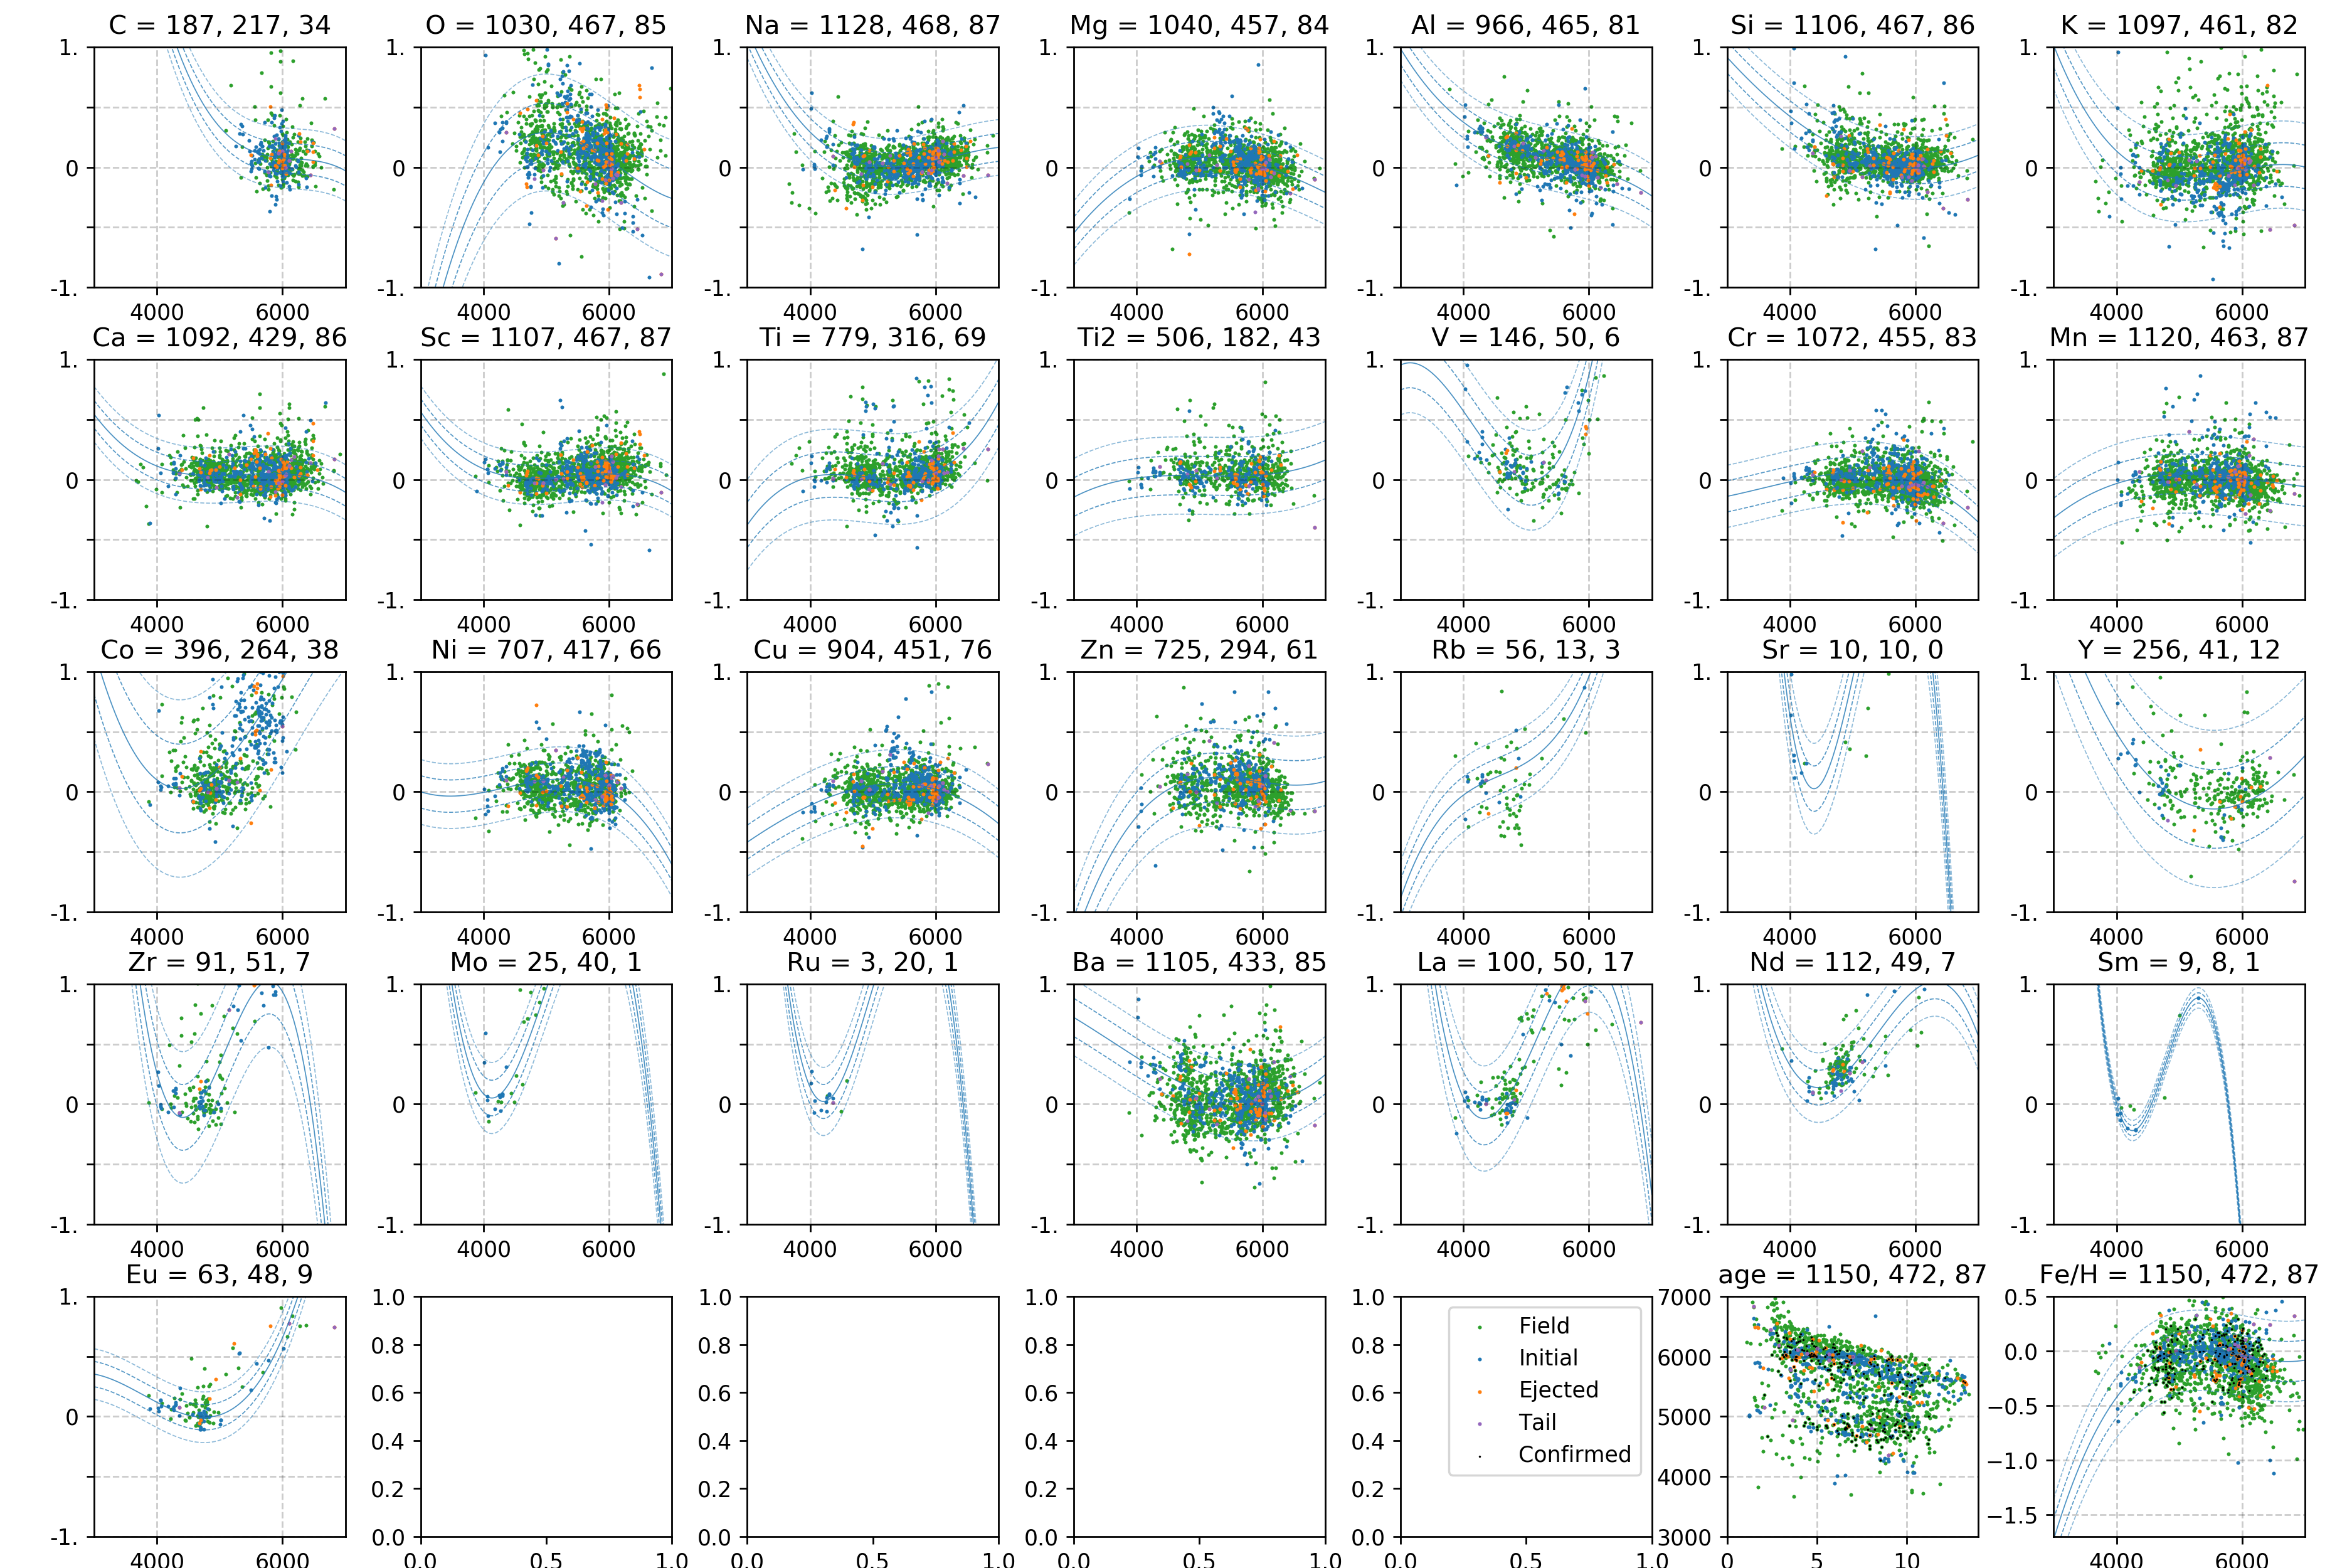
\includegraphics[width=\textwidth]{p_teff_abundances_NGC_2682_orbits_DR3_new_flag0.png}
	\caption{NGC 2632 abundance scatter plots as a function of effective stellar temperature. The solid blue line represents the best fit on the cluster population. The 1$\sigma$ and 2$\sigma$ abundance deviations from the fit are given by dashed blue lines of decreasing intensity. Coloured dots represent filed (green), members (blue), and possibly ejected (orange) stars. Their number is given above every panel, following the elements' name. Purple dots preset known tails of slowly evaporating stars in some clusters. The last two panel present \Teff\ of stars at different ages, and dependence of \Feh\ on their \Teff. The black dots in those two panels indicate possibly ejected stars whose chemistry was matched to cluster stars.}
	\label{fig:ct_cluster1}
\end{figure}

\begin{figure}
	\centering
	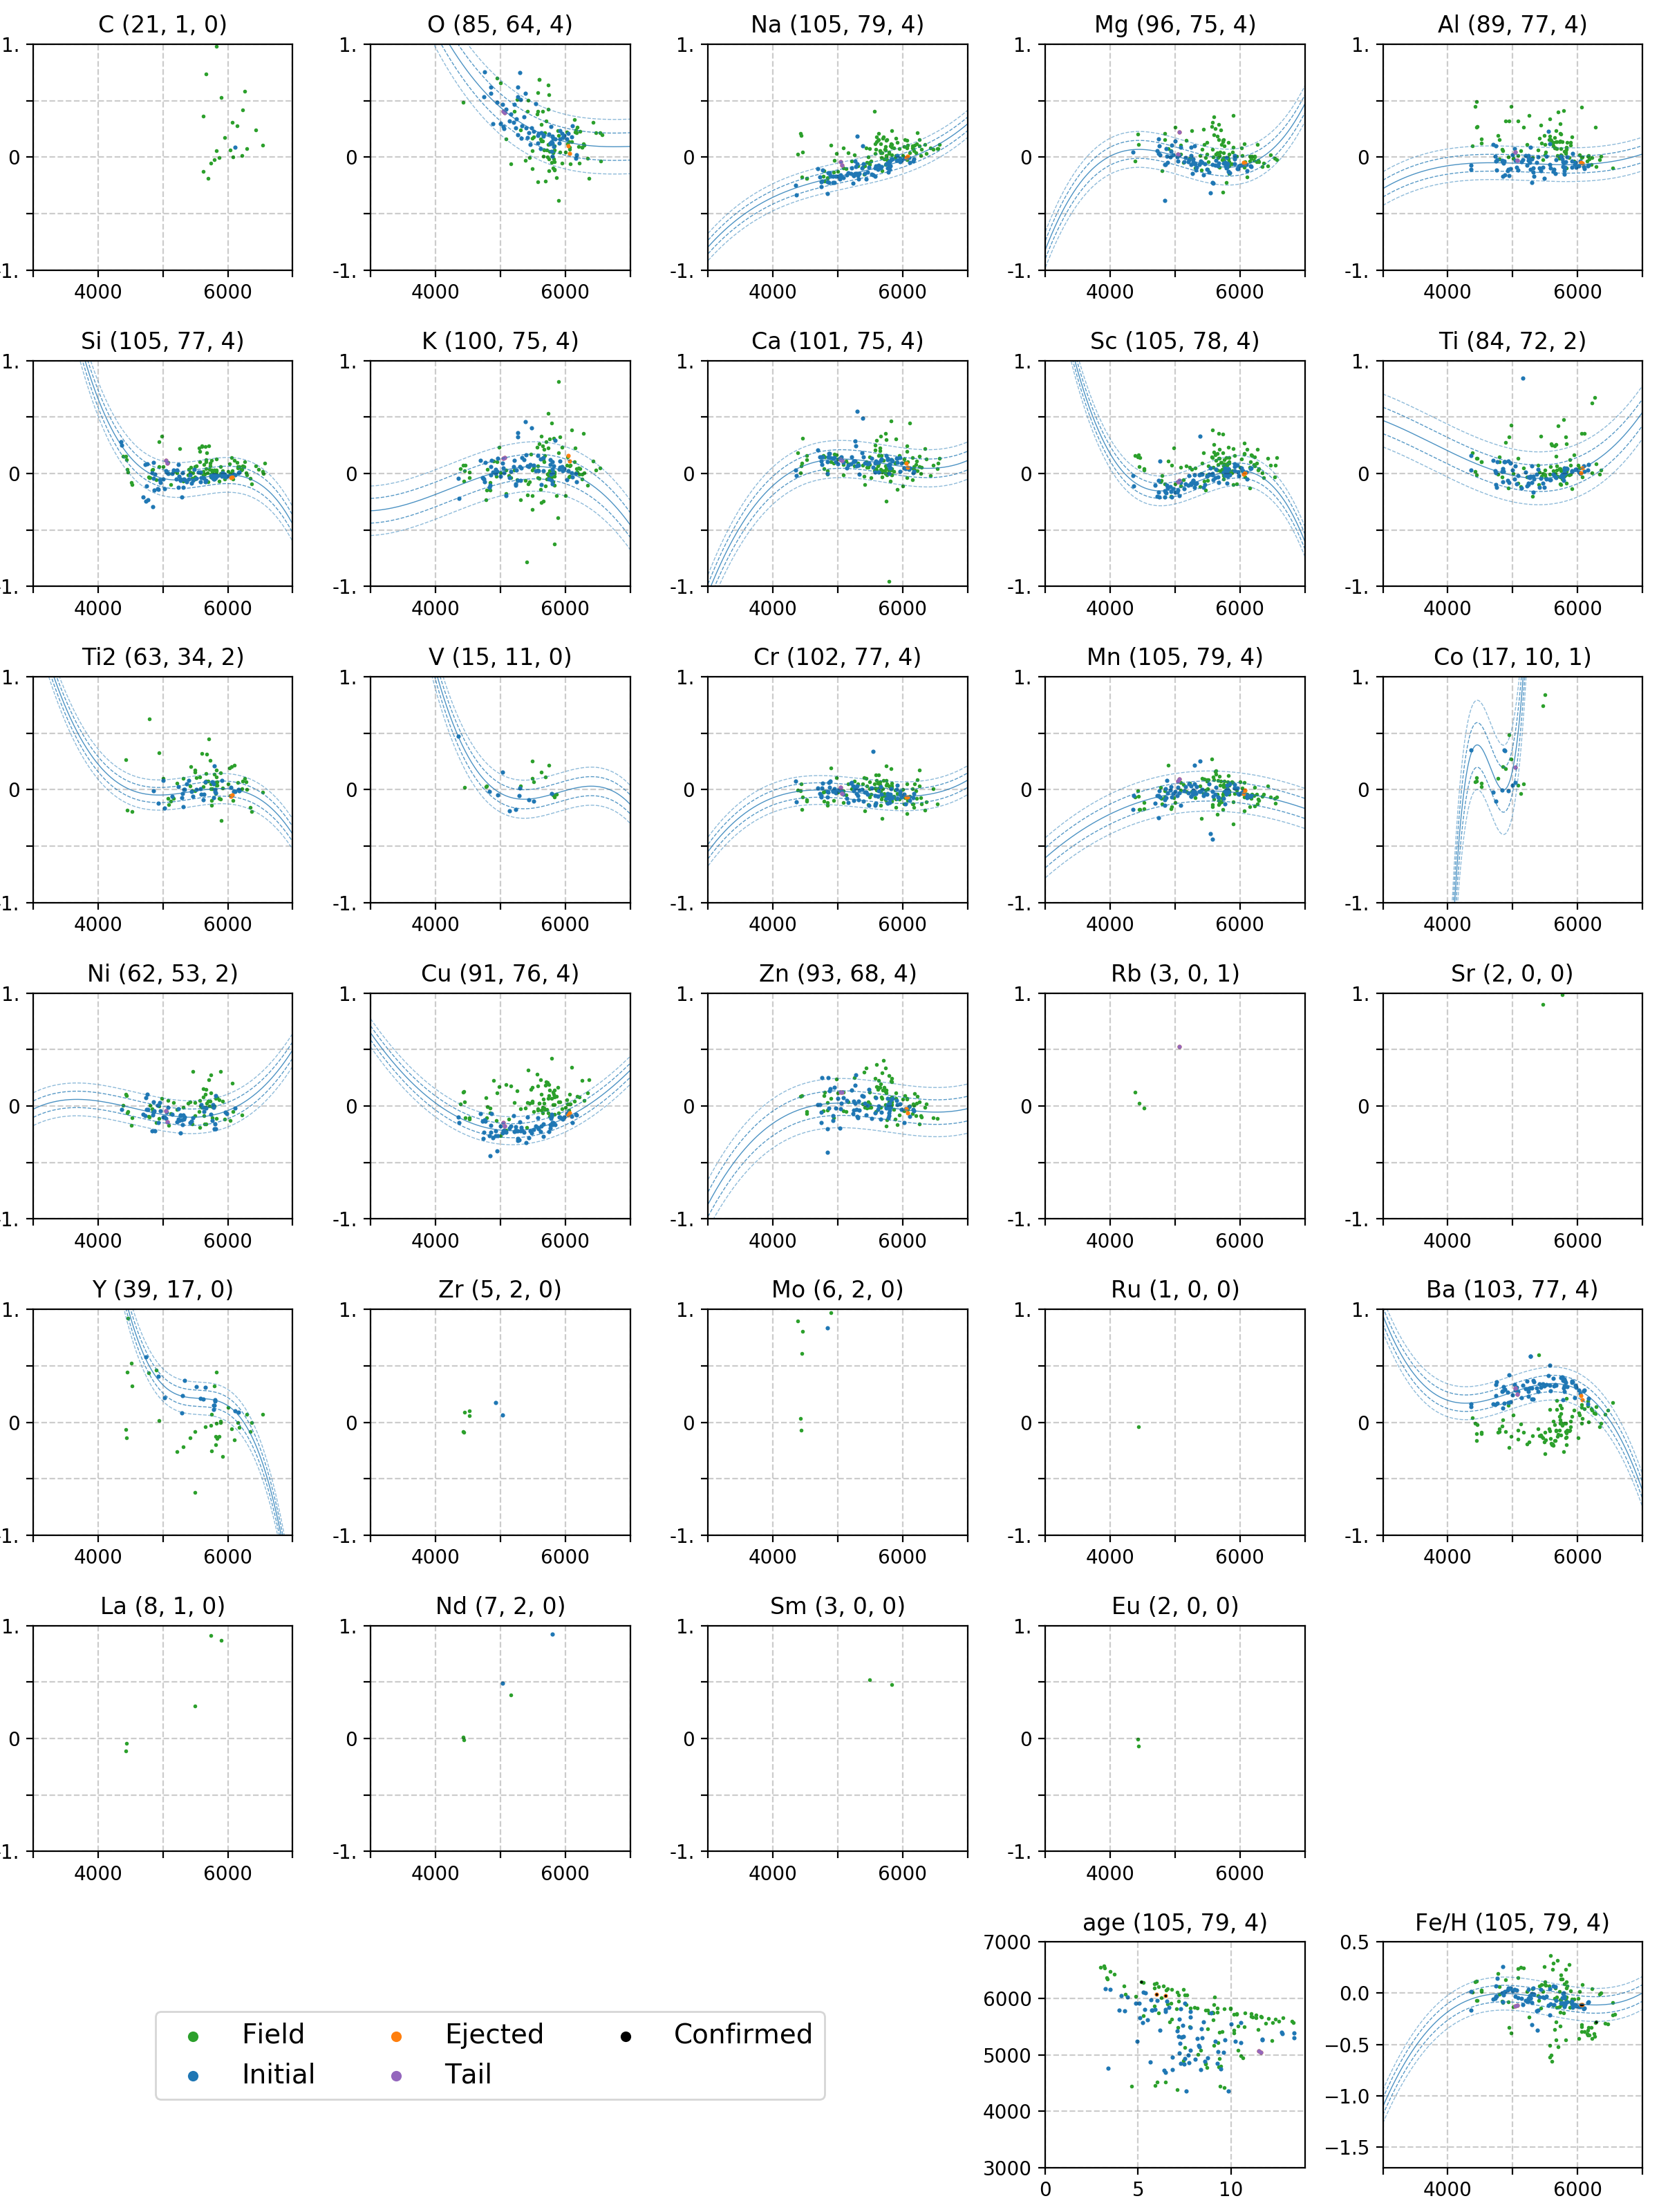
\includegraphics[width=\textwidth]{p_teff_abundances_Blanco_1_orbits_DR3_new_flag0.png}
	\caption{Same plots as in Figure \ref{fig:ct_cluster1} but for open cluster Blanco 1.}
	\label{fig:ct_cluster2}
\end{figure}

\begin{figure}
	\centering
	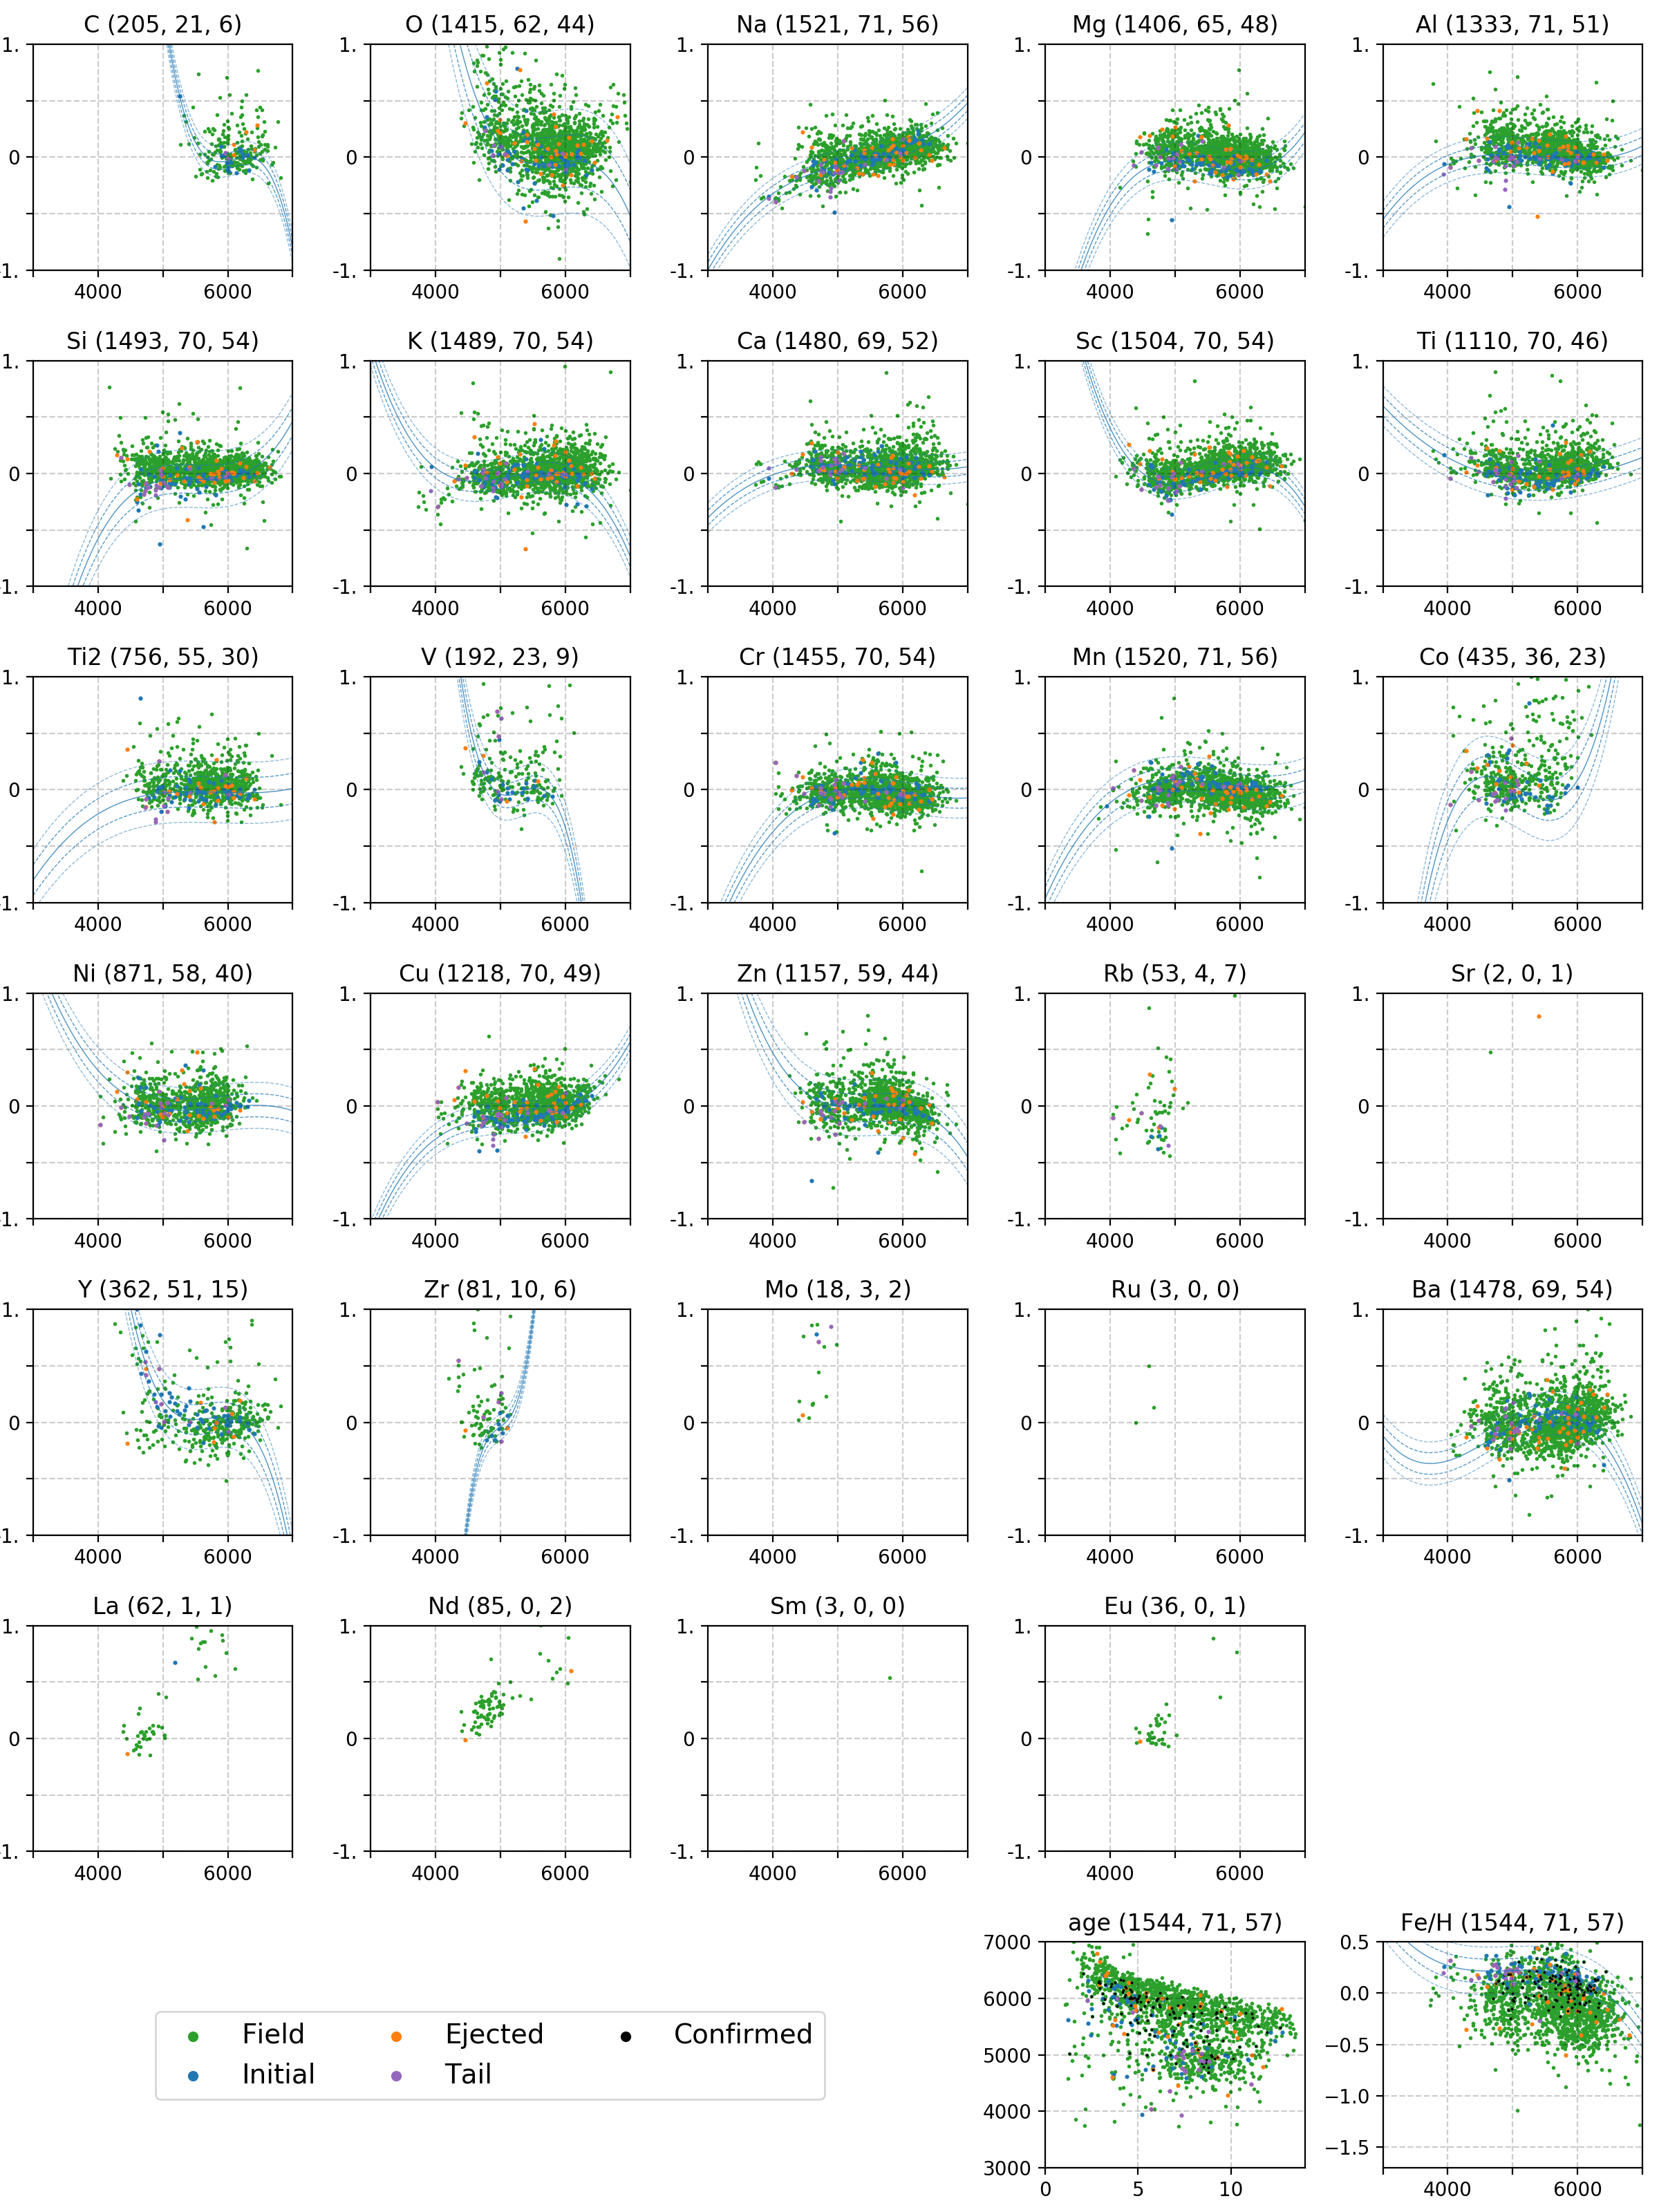
\includegraphics[width=\textwidth]{p_teff_abundances_NGC_2632_orbits_DR3_new_flag0.png}
	\caption{Same plots as in Figure \ref{fig:ct_cluster1} but for open cluster NGC 2632.}
	\label{fig:ct_cluster3}
\end{figure}

\begin{figure}
	\centering
	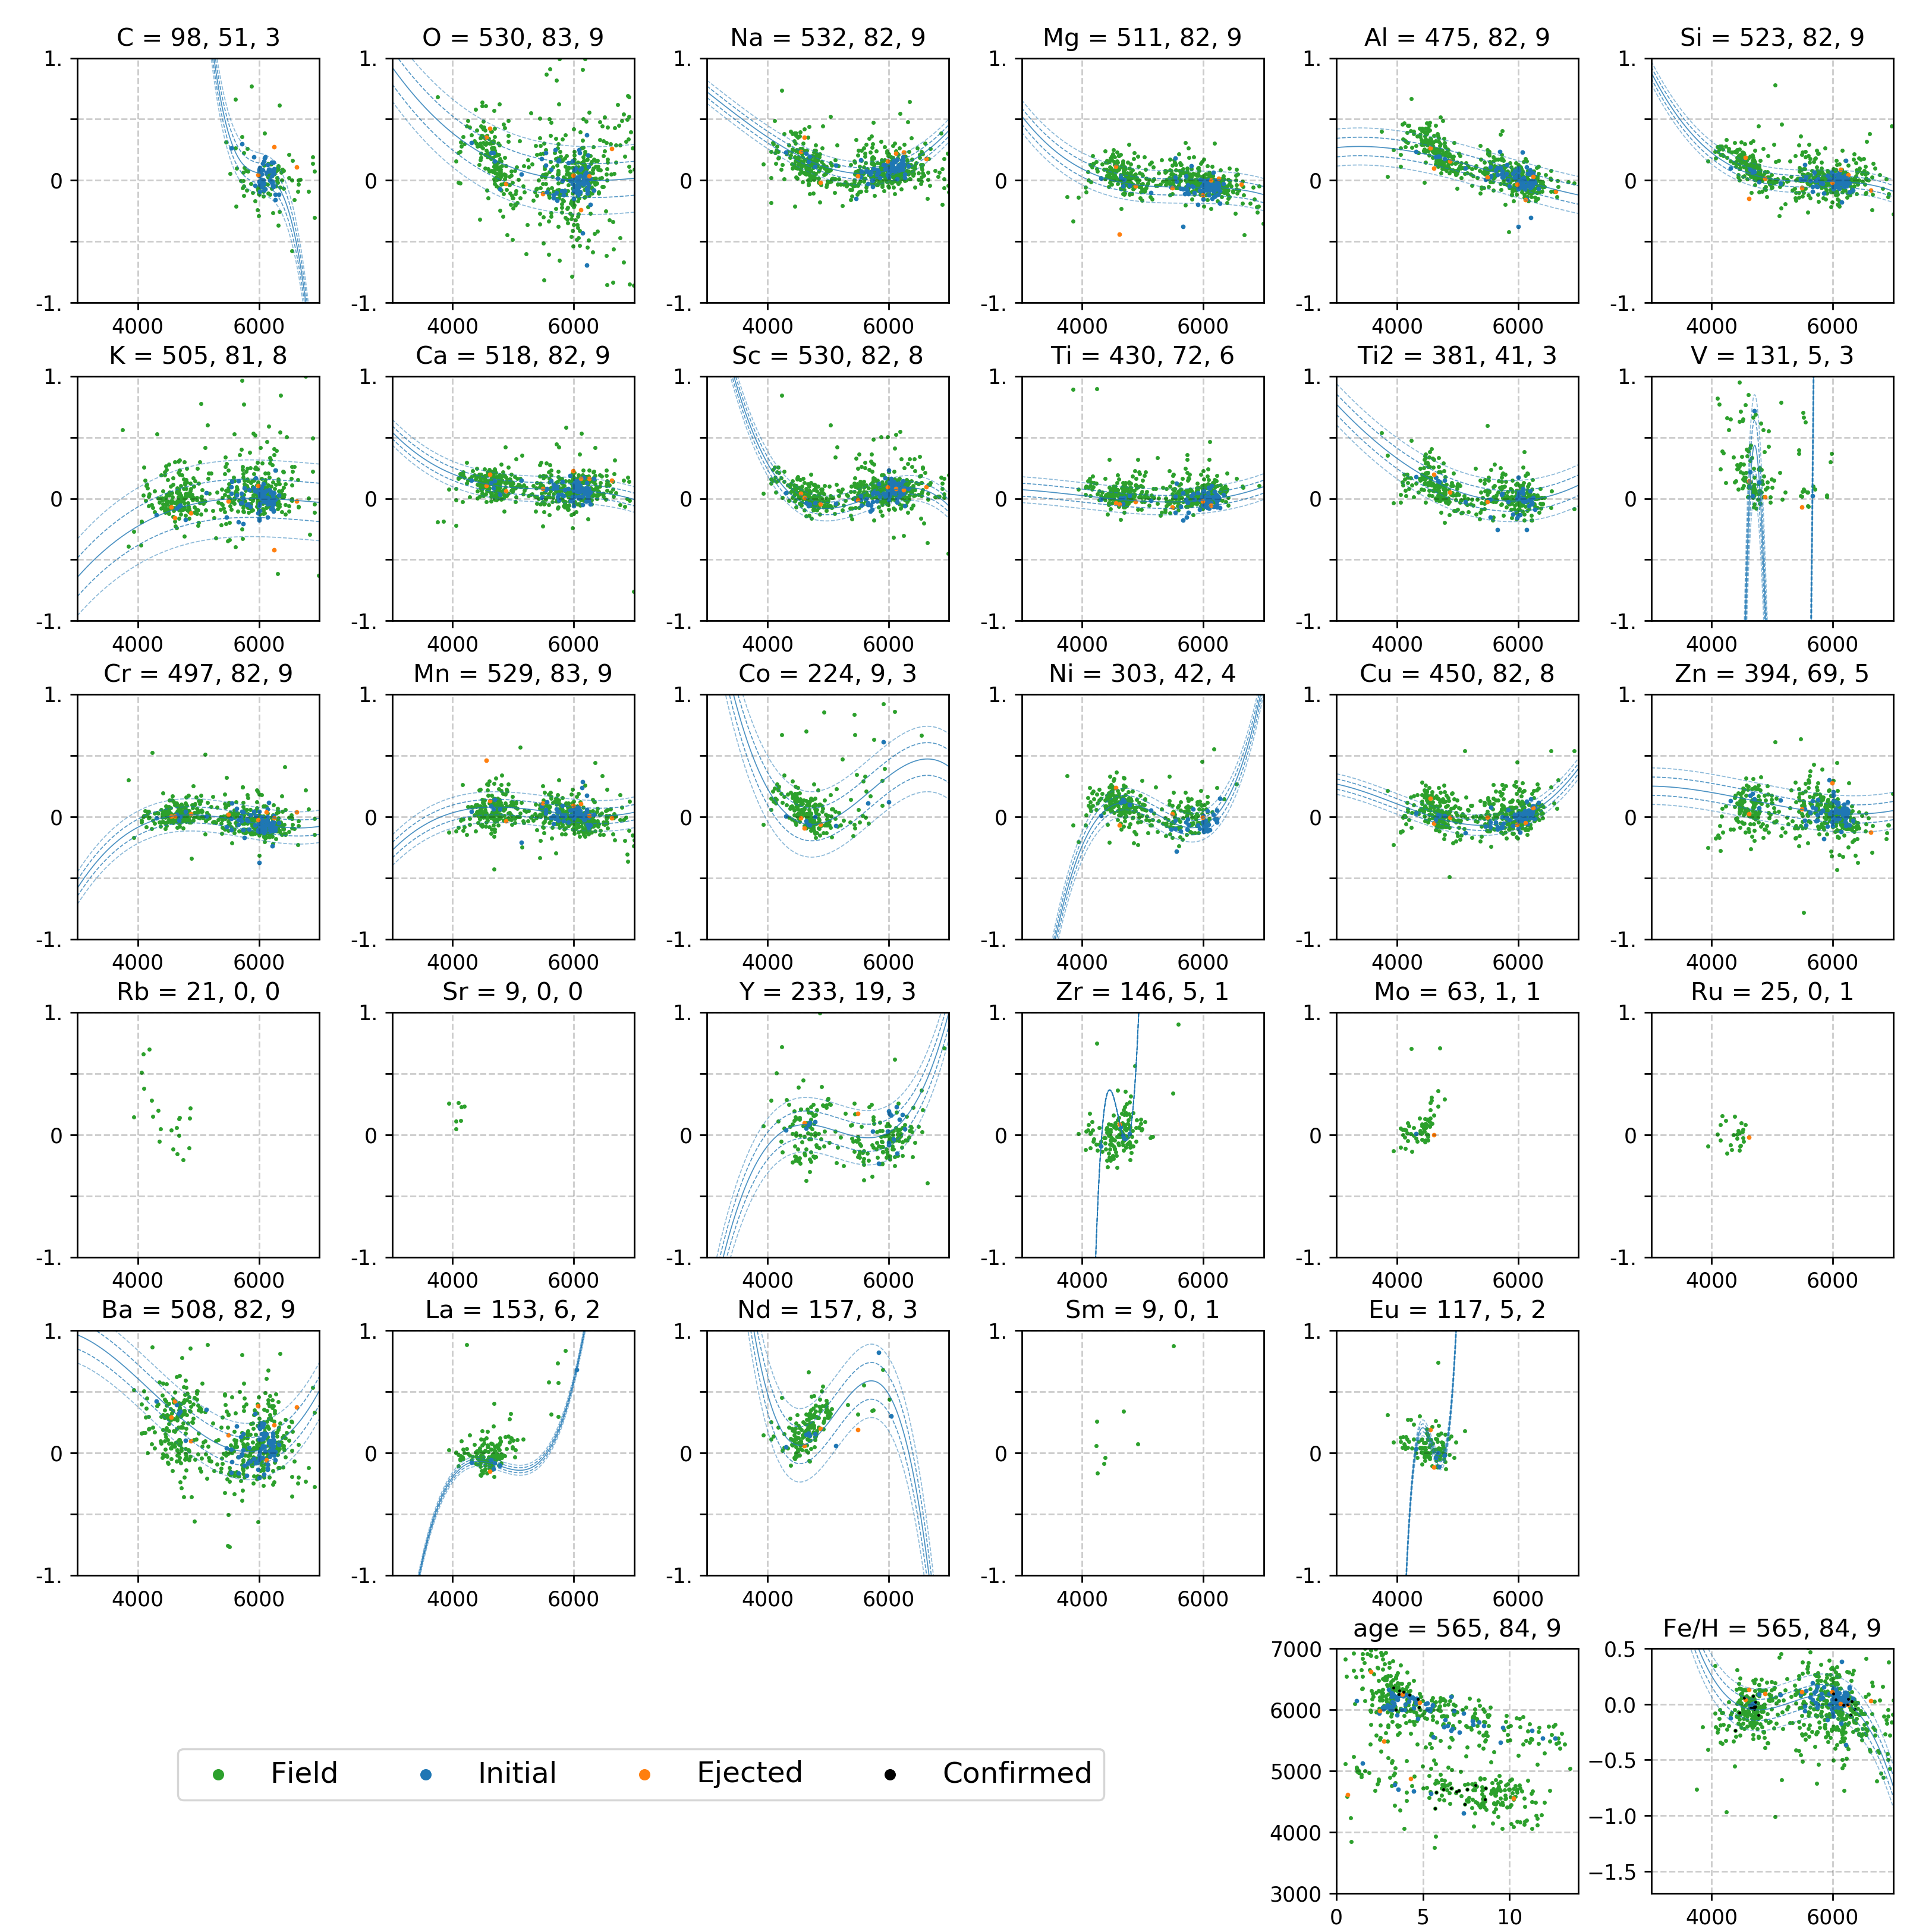
\includegraphics[width=\textwidth]{p_teff_abundances_Ruprecht_147_orbits_DR3_new_flag0.png}
	\caption{Same plots as in Figure \ref{fig:ct_cluster1} but for open cluster Ruprecht 147.}
	\label{fig:ct_cluster4}
\end{figure}

\begin{table}
	\centering
	\caption{The number of acquired the \Gh\ spectra among different cluster components that were considered during the chemical comparison. No parameter or abundance flagging was yet used at this point. Stars represented by these statistics are a subset of stars given in Table \ref{tab:cluster_stats}. Because of a small percentage of repeated observations, few clusters (especially NGC 2682 that was used as the calibration and verification filed) can have a higher number of spectra than the number of member stars.}
	\begin{tabular}{l | c | c | c }
		\hline
		Cluster & Field & Ejected & Members \\
		\hline
		Berkeley 32  & 0 & 0 & 0 \\ 
		Blanco 1     & 0 & 0 & 0 \\
		IC 4665      & 0 & 0 & 0 \\
		Mamajek 4    & 0 & 0 & 0 \\
		Melotte 22   & 0 & 0 & 0 \\
		Melotte 25   & 0 & 0 & 0 \\
		NGC 1817     & 0 & 0 & 0 \\
		NGC 1901     & 0 & 0 & 0 \\
		NGC 2112     & 0 & 0 & 0 \\
		NGC 2204     & 0 & 0 & 0 \\
		NGC 2516     & 0 & 0 & 0 \\
		NGC 2548     & 0 & 0 & 0 \\
		NGC 2632     & 0 & 0 & 0 \\
		NGC 2682     & 0 & 0 & 0 \\
		NGC 6253     & 0 & 0 & 0 \\
		Ruprecht 147 & 0 & 0 & 0 \\
		\hline
	\end{tabular}
	\label{tab:cluster_stats_abund}
\end{table}

\subsection{Abundance trends}
\label{sec:abund_trends}
%Ker vidimo in tudi drugi modeli kar mocne trende zastopanosti v odvisnosti od fizikalnih parametrov zvezd, je treba te nekako spraviti na isto raven. Najlazje diferencialno - naredimo fit na kopico in gledamo koliko ostali odstopajo od tega
One of the first things we noticed on the shown abundance scatter plots is their strong dependence with physical parameters, especially \Teff. As this is not the first or unique observation of those trends \cite{2010A&A...523A..71G, 2013ApJ...775...58B, 2016MNRAS.457.3934L, 2018A&A...619A.176B, 2019arXiv191208539C}, they are most likely partial products of insufficient/inaccurate stellar models and/or actual abundance patterns, and not induced solemnly by the employed \SME\ spectrum analysis pipeline described that was used by \citet{buder2020} to determine stellar abundances.

If we presume that observed trends are artificially induced and considered cluster members should have a homogeneous chemical composition that is independent of stellar type, a differential chemical tagging analysis can be used \cite{2019arXiv191208539C}. Such analysis considers only comparisons among stars with a similar set of stellar parameters. To describe observed trends, we independently fitted a 3$^{rd}$ degree polynomial function using $2.5\sigma$ clipping algorithm in 2 steps to every abundance versus \Teff\ diagram. By subtracting fitted trends, we estimated degree of intracluster scatter for every element. Because of limitations of measuring certain abundances, the fit was not performed if the number of valid abundance measurements was lower or equal to a used polynomial degree $+1$.

%Nekam lahko morda pride se primerjava razprsenosti zastopanosti med posameznimi elementi in posameznimi kopicami.

\subsection{Chemical membership}
\label{sec:chem_ej_tag}
%Pogledamo trende in fite, ter koliko moznih izvzenih zvezd se poraja in sklada s temi kemicnimi trendi. Morda nek threshold koliko je dobrih oziroma skladnih s samo kopico, saj ima tudi ta le kar nekaj razpona v izmerjenih/izracunanih vrednostih parametrov.
Having an analytical description of an individual abundance behaviour for every cluster, we can estimate how many and how accurately do the identified ejected stars match with cluster abundance patterns and trends. The most straightforward way to perform this is to count how often does abundance value of an investigated star fall inside a $1\sigma$ (or $2\sigma$ for a more relaxed selection) region around an abundance trend. Both regions and fitted trends are visualised in Figures \ref{fig:ct_cluster1}, \ref{fig:ct_cluster2}, \ref{fig:ct_cluster3}, and \ref{fig:ct_cluster4}. Before performing such counting, we additionally omitted abundance trends of the following chemical elements: V, Rb, Sr, Y, Zr, Mo, Ru, La, and Sm. Their low number of successful measurements per cluster and uncertain trends were not beneficial to the whole chemical tagging experiment and influenced only a small fraction of stars. \rb{nacelona tega sploh ne zelimo delat, samo eni so vizualno res cudni} A star was counted as chemically similar if it matched (e.g. fell inside selected $\sigma$ region around the fitted trend line) to a cluster in at least $68$\% of considered abundances.

\subsection{Tagging remaining field stars}
\label{sec:chem_fi_tag}
%Kaj se zgodi ce iste kemicne informacije in thresholde uporabimo se za ostale analizirane zvezde v bljizini. Dobimo sploh kaj zvezd ven iz tega in kaksen bi bil v tem primeru njihov kinematicni vektor.
The same principle can also be applied to remaining nearby field stars. As clearly evident from Figures \ref{fig:ct_cluster1}, \ref{fig:ct_cluster2}, \ref{fig:ct_cluster3}, and \ref{fig:ct_cluster4}, the cluster abundances are mostly similar to field stars and lie close to their densest regions in a scatter plot. Therefore, we were interested into the probability of a field star being chemically similar to a nearby cluster. In contrast, some of the investigated clusters, especially Blanco 1, showed evident signs of being chemically separable from neighboring populations in few abundances that are commonly used as chemical tracers of galactic evolution and stellar age \citep{2003A&A...410..527B, 2018MNRAS.474.2580S, 2020MNRAS.491.2043L}.

For a field chemical tagging procedure, we used the same selection principle as previously described in Section \ref{sec:chem_ej_tag}. The results of both tagging experiments are presented in Table \ref{tab:cluster_stats_abundtag}.

\begin{table}
	\centering
	\caption{Number and percentage of all considered and chemically similar (tagged) stars in the spatial neighborhood around analysed open clusters. Percentages indicate number of stars in different components that are similar to cluster abundance pattern and scatter. Selection algorithm is detailed in Section \ref{sec:chem_ej_tag}. Only spectra with unflagged stellar parameters were used to produce shown statistics.}
	\begin{tabular}{l | c | c | c | c }
		\hline
		Cluster & \multicolumn{2}{c}{Ejected}  & \multicolumn{2}{c}{Field} \\
		 & All & Tagged & All & Tagged \\
		\hline
		Berkeley 32  & 2 & 0 (0.0\%) & 39 & 0 (0.0\%) \\ 
		Blanco 1     & 4 & 2 (50.0\%) & 99 & 3 (3.0\%) \\
		IC 4665      & 4 & 0 (0.0\%) & 905 & 0 (0.0\%) \\
		Mamajek 4    & 25 & 7 (28\%) & 2273 & 136 (6.0\%) \\
		Melotte 22   & 10 & 1 (10\%) & 708 & 76 (10.7\%) \\
		Melotte 25   & 12 & 4 (33.3\%) & 639 & 4 (10.6\%) \\
		NGC 1817     & 6 & 0 (0.0\%) & 427 & 6 (1.4\%) \\
		NGC 1901     & 19 & 4 (21.1\%) & 5510 & 1034 (18.8\%) \\
		NGC 2112     & 4 & 0 (0.0\%) & 268 & 8 (3.0\%) \\
		NGC 2204     & 19 & 3 (16.7\%) & 113 & 14 (12.4\%) \\
		NGC 2516     & 70 & 4 (5.7\%) & 3285 & 72 (2.2\%) \\
		NGC 2548     & 5 & 0 (0.0\%) & 603 & 6 (1.0\%) \\
		NGC 2632     & 56 & 7 (12.5\%) & 1523 & 74 (4.9\%) \\
		NGC 2682     & 85 & 32 (37.6\%) & 1133 & 253 (22.3\%) \\
		NGC 6253     & 27 & 3 (11.1\%) & 648 & 28 (4.3\%) \\
		Ruprecht 147 & 9 & 0 (0.0\%) & 559 & 23 (4.1\%) \\
		\hline
	\end{tabular}
	\label{tab:cluster_stats_abundtag}
\end{table}

\section{Comparison with known remains}
\label{sec:tails_chem}
%Izvedli bi krajso primerjavo kako v luci nasih dognanj vidimo plimske repe kopic, ki so jih zaznali drugi.
In the previous section we analysed stars whose orbits indicate that they could be ejected from open clusters sometime in their past. Depending on a mass of involved stars and their proximity during the slingshot mechanism, stars could be thrown out of the cluster into inter-stellar space at various velocities and directions. 

A less energetic and more gradual mechanism that also influences lifetime of an open cluster is tidal stripping of stars \citep{2006A&A...455L..17L}. It happens during clusters' journey trough more heavily populated regions such as spiral arms. In this section we compare kinematics and chemical composition of known tidal structures \citep[discovered in \Gs\ data by ][]{2019AA...627A...4R, 2019AA...627A.119C, 2019AA...621L...3M, 2019arXiv191206657Z} of a few \Gh\ clusters with other previously analysed structures.

\subsection{Kinematics comparison}
Ali je njihova kinematika sploh taksna da integracija njihovi orbit kaze nazaj proti volumnu kopice ali pac ne. Ce ne, imamo morda neko potrditev da res isceno izvrzene in ne strukture nekih pocasnih gravitacijskih vplivov??

First we compared their measured kinematics and position to determine if it would be possible to select the same subset only on those properties, without prior knowledge that they might once be a part of a nearby dissolving open cluster. \rb{nisem se kaj veliko tega gledal}

\subsection{Tidal tails chemistry}
Kaj pa pravi njihova kemicna sestava na povezavo s kopico in ali imajo enake galah podpise? Ce ne, se je treba spomnit kaj pametnega zakaj bi lahko temu bilo tako. Ne deluje teorija, analiza nasih podatkov ali pa pac niso bili formirani ob istem casu.

Among randomly acquired The \Gh\ spectra, we observed some stars that where identified to belong to kinematically discovered tidal structures around open clusters.

For a tidal tail chemical tagging procedure, we used the same selection principle as previously described in Section \ref{sec:chem_ej_tag}. The result of the tagging experiment is presented in Table \ref{tab:cluster_stats_tails}.

\begin{table}
	\centering
	\caption{Opis te tabele. Tabela se v delu.}
	\begin{tabular}{l | c | c | c | c | c | r }
		\hline
		Cluster & Stars in & Without used & Common with & \Gh\ unflagged & Chemically & Tail membership\\
		 & reference & cluster members & ejected & parameters (\% in & tagged & reference\\
		 &  &  & (\% of ejected) & common with ejected) & (\% of valid) & \\
		\hline
		Blanco 1     & 644 & 276 & 4 (27\%) & 2 (100\%) & 0 (0\%) & \citet{2019arXiv191206657Z} \\
		NGC 2632  & 1393 & 738 & 37 (22\%) & 22 (68\%) & 0 (0\%) & \citet{2019AA...627A...4R} \\
		NGC 2682     & 952 & 241 & 20 (9\%) & 16 (81\%) & 0 (0\%) & \citet{2019AA...627A.119C} \\
		NGC 1817     & 0 & 0 & 0 (0\%) & 0 (0\%) & 0 (0\%) & \citet{a} \\
		Melotte 22   & 0 & 0 & 0 (0\%) & 0 (0\%) & 0 (0\%) & \citet{a} \\
		Melotte 25   & 0 & 0 & 0 (0\%) & 0 (0\%) & 0 (0\%) & \citet{2019AA...621L...3M} \\
		\hline
	\end{tabular}
	\label{tab:cluster_stats_tails}
\end{table}

\section{Summary}
\label{sec:clusters_summary}

\section{Conclusions}
\label{sec:clusters_conclusions}
